% fig_confidence.tex
% Composite confidence score gamma vs Rf
% Curves: 3PH (solid blue), SLG (dashed red)
% Acceptance threshold gamma_min = 0.80 (from hif_sim.py)
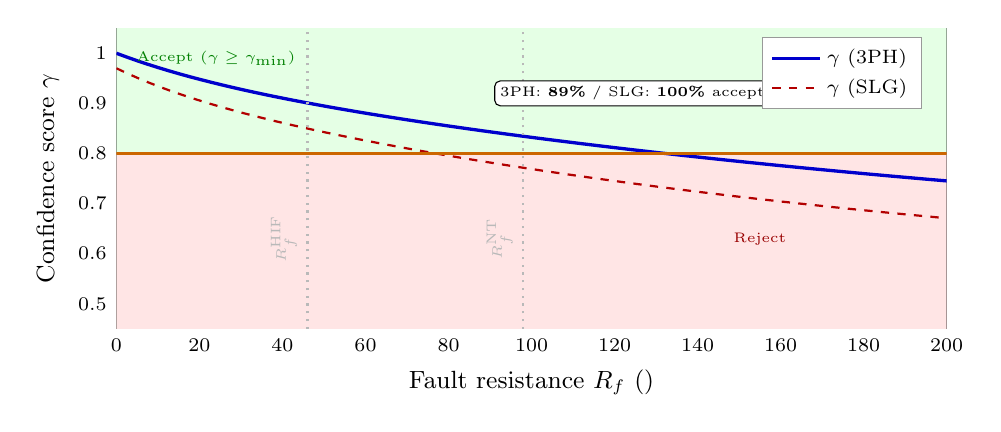
\begin{tikzpicture}
\begin{axis}[
  width=\columnwidth, height=5.4cm,
  xlabel={Fault resistance $R_f$ (\si{\ohm})},
  ylabel={Confidence score $\gamma$},
  xmin=0, xmax=200,
  ymin=0.45, ymax=1.05,
  ytick={0.5,0.6,0.7,0.8,0.9,1.0},
  grid=both,
  grid style={gray!25,line width=0.3pt},
  tick label style={font=\scriptsize},
  label style={font=\small},
  legend style={at={(0.97,0.97)},anchor=north east,
                font=\scriptsize,fill=white,draw=black!40},
  clip=true]

  % Accept region
  \addplot[fill=green!10,draw=none,forget plot]
    coordinates {(0,0.80)(200,0.80)(200,1.05)(0,1.05)} \closedcycle;
  % Reject region
  \addplot[fill=red!10,draw=none,forget plot]
    coordinates {(0,0.45)(200,0.45)(200,0.80)(0,0.80)} \closedcycle;

  % Synthetic gamma curve 3PH
  \addplot[blue!80!black,very thick,samples=80,domain=0:200]
    { 0.57 + 0.39*exp(-x/250) + 0.04*exp(-x/25) };
  \addlegendentry{$\gamma$ (3PH)}

  % Synthetic gamma curve SLG
  \addplot[red!70!black,thick,dashed,samples=80,domain=0:200]
    { 0.52 + 0.41*exp(-x/200) + 0.04*exp(-x/20) };
  \addlegendentry{$\gamma$ (SLG)}

  % Acceptance threshold
  \draw[orange!80!black,thick]
    (axis cs:0,0.80) -- (axis cs:200,0.80)
    node[right,font=\tiny,orange!80!black] {$\gamma_{\min}=0.80$};

  % Regime markers
  \draw[gray!55,dotted,thick]
    (axis cs:46,0.45) -- (axis cs:46,1.05)
    node[above,rotate=90,font=\tiny,gray!55,pos=0.3]
    {$R_f^{\mathrm{HIF}}$};
  \draw[gray!55,dotted,thick]
    (axis cs:98,0.45) -- (axis cs:98,1.05)
    node[above,rotate=90,font=\tiny,gray!55,pos=0.3]
    {$R_f^{\mathrm{NT}}$};

  % Region labels
  \node[font=\tiny,green!50!black]
    at (axis cs:24,0.99) {Accept ($\gamma \geq \gamma_{\min}$)};
  \node[font=\tiny,red!60!black]
    at (axis cs:155,0.63) {Reject};

  % Acceptance rate annotation
  \node[draw,fill=white,rounded corners=2pt,inner sep=2pt,
        font=\tiny,align=center]
    at (axis cs:140,0.92)
    {3PH: \textbf{89\%} / SLG: \textbf{100\%} acceptance ($\gamma\geq0.80$)};

\end{axis}
\end{tikzpicture}
